\newpage

\section{introduction}

Durant le 20eme siécle la course à l'espace a permis l'evolution de nombreuses entreprises, le developpement de nouveaux materiaux adapté comme la fibre de carbone (cf lucas), un progression dans le dimensionnement et l'élaboration de nouveaux systeme electronique et de grande avancé iformatique.\\
Au 21eme siécle de nouveaux projet spaciaux emergent au 4 coins du globe. Ces projets ou mission spatial permettent l'emergence de nouvelles technologie pour répondre à plusisuers defis, telque la mise en orbite de nouveaux satellite (ref), l'exploration de nouvel astéroide(ref), la rentree dasn l'atmospheres d'une planete lointaine comme mars avec la projet Apollo(ref). C'est problématique amenent à concevoir de nouveau vehicule spaciaux plus performant, menant des missions au traveurs l'espace comme le X-37B ou bien la conception de Space rider ressanblnt à L' IXV qui a réalisé son unique vol en février 2015.\\

\begin{figure}[h!]
 \centering
 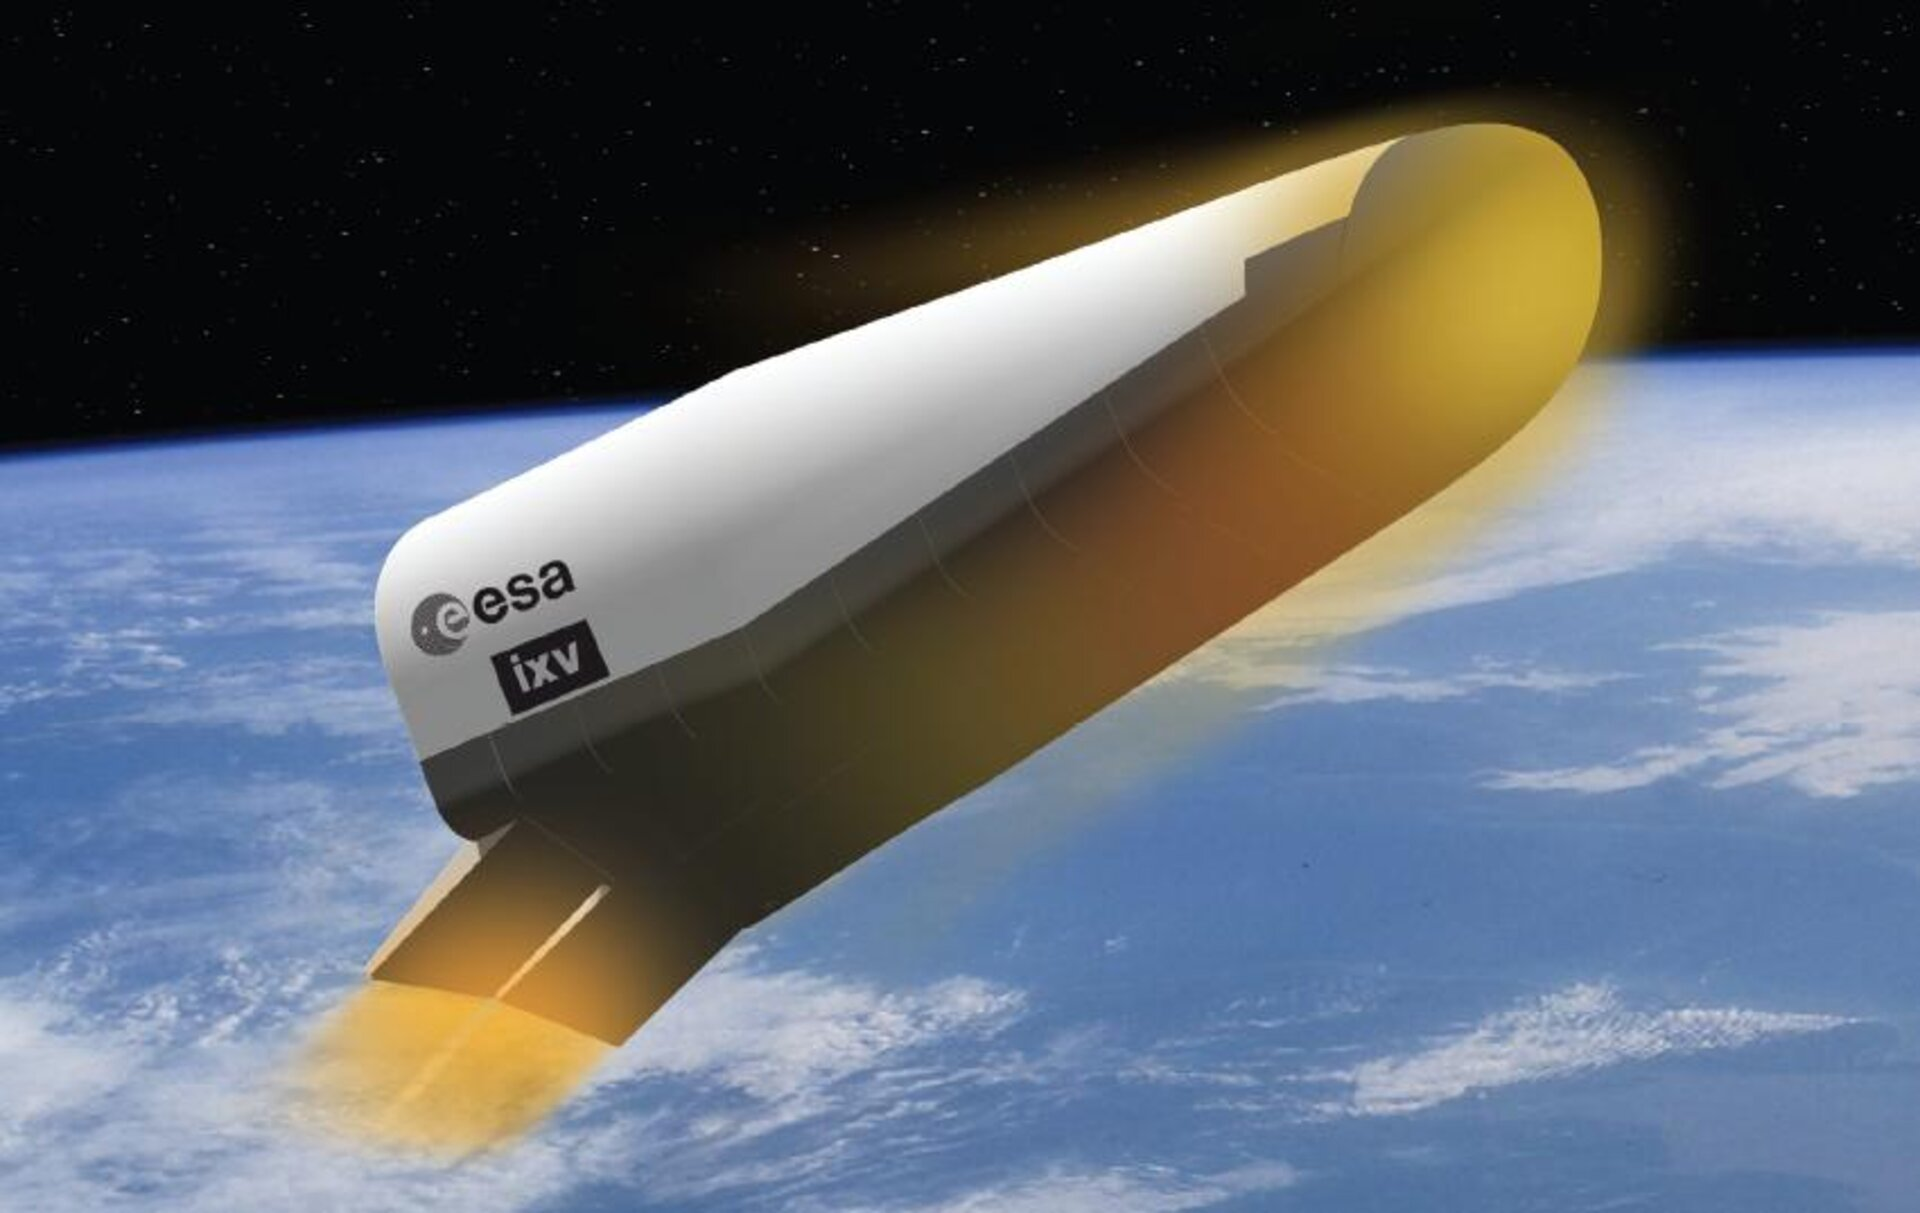
\includegraphics[width=0.6\linewidth]{chapter1_introduction/pictures/IXV_pillars.jpg}
 \vspace{-2ex}
 \caption{IXV spatial navette by esa}
  \vspace{2ex}
 \label{IXV}
\end{figure}

Contrairement à l'époque ou les essais en vol etait courrant, le dimmensionnment des nouveaux systeme, que ce soit électronique au du design, sans ommetre le comportement thermique des materiaux choisis des vehicule spaciaux reposent essentiellment sur la simulations numerique beaucoup moins couteuse.\\
Pour produire de nouveaux design de veicule pur nos missions spatial, il faut étuider les écoulement fluide autour de ces corps astraux.
L’étude des écoulements fluides qui composent notre environnement est
un sujet qui suscite un grand intérêt et qui n’est pourtant pas encore arri-
vée à maturité. Ce domaine physique est extrement compliqué à etudier notament u au equations de navier stokes chercahnt encore à etre prouver et qui est une des question millinaires existante.\\
Lors d'une rentree atmopherique les vehicules sont soumis à des forces de pression d'énormes, avec de fort gradient de température sur les parois. Deplus
lors de vls a grande vitesses plusieurs phenomene complexes apparaissent commes des choc ou detentes à fort gradient de pression et de densité. Il faut alors réusir à simuler ces phenomemene complexes avec precisions et capturer les differentes variables  à la paois. Deplus la simulation d'écoulemnt 2D, bien que utile ne permet pas de modeliser des phenomene comme la turbulence qui n'est calculé que en 3D. c'est dans ce contexte précis qu' il est necessaire de developpé de nouveaux code de calcule 3D, massivememtn parrallem permettant de\\
a new simulation code in the context of fast design of atmospheric reentry vehicles. To do so, we must develop a 3D simulation code and run simulations.




